\documentclass[a4paper,12pt]{article}


%%%%%%%%%%%%%%%%%%%%%%%%%%%%%%%%%%%%%%%%%%%%%%%%%%%%%%%%%%%%
% DELIVERABLE META DATA
%
% Modify so that the meta data is correct for this deliverable.
%%%%%%%%%%%%%%%%%%%%%%%%%%%%%%%%%%%%%%%%%%%%%%%%%%%%%%%%%%%%

% The WP to which the deliverable belongs (the x in Dx.y).

\def\nlafetMajor{6}

% The deliverable number within the WP (the y in Dx.y).

\def\nlafetMinor{4}

% A long title for the deliverable (for the front page).
%
% Look up the correct title in the grant agreement.

\def\nlafetTitle{An Off-line Autotuning Framework based on Heuristic Search}

% A short title for the deliverable (for the header).
%
% Shorten the title if necessary to fit the header.

\def\nlafetShortTitle{Off-line Autotuning}

% The month when this version was published.

\def\nlafetMonth{March}

% The year when this version was published.

\def\nlafetYear{2017}

% The scheduled delivery of this deliverable.
%
% This is the last day of the delivery month found in the grant
% agreement. November 2015 is referred to as M1. For example, if the
% delivery month is M6, then the date below should read 2016-04-30
% since April 2016 is M6.

\def\nlafetScheduledDelivery{2017-04-31}

% The actual delivery of this deliverable.
%
% This is the date the deliverable was actually delivered. Do not
% change this field until the actual delivery.

\def\nlafetActualDelivery{(not yet delivered)}

% The current major and minor version number of this document.
%
% The bigger the number, the newer the version. How you assign major
% and minor version numbers is up to you. The sole purpose of the
% version number is to make it easier to reference different versions.

\def\nlafetVersionMajor{0}
\def\nlafetVersionMinor{1}

% The short name (UMU/UNIMAN/STFC/INRIA) of the partner responsible
% for this deliverable.

\def\nlafetResponsiblePartner{UNIMAN}

% The dissemination level.
%
% Either public or confidential. Look up the correct level in the the
% grant agreement.

% \def\nlafetDisseminationLevel{PU --- Public}
\def\nlafetDisseminationLevel{CO --- Confidential}






%%%%%%%%%%%%%%%%%%%%%%%%%%%%%%%%%%%%%%%%%%%%%%%%%%%%%%%%%%%%
% PACKAGES REQUIRED BY TEMPLATE
%
% Do not touch!
%%%%%%%%%%%%%%%%%%%%%%%%%%%%%%%%%%%%%%%%%%%%%%%%%%%%%%%%%%%%

% Input and font encoding.
\usepackage[utf8]{inputenc}
\usepackage[T1]{fontenc}
\usepackage{lmodern}

% Colored table.
\usepackage{xcolor}
\usepackage{colortbl}

% Graphics.
\usepackage{graphicx}

% Header/footer.
\usepackage{fancyhdr}

% Margins.
\usepackage[margin=25mm]{geometry}

% Total page count.
\usepackage{lastpage}

% URL typesetting.
\usepackage{url}

% Table with word wrap.
\usepackage{tabularx}


\usepackage{amsmath,amssymb}





%%%%%%%%%%%%%%%%%%%%%%%%%%%%%%%%%%%%%%%%%%%%%%%%%%%%%%%%%%%%
% HEADER / FOOTER
%
% Do not touch!
%%%%%%%%%%%%%%%%%%%%%%%%%%%%%%%%%%%%%%%%%%%%%%%%%%%%%%%%%%%%

\pagestyle{fancy}
\renewcommand{\footrulewidth}{\headrulewidth}
\lhead{\bf NLAFET}
\rhead{\bf D\nlafetMajor.\nlafetMinor: \nlafetShortTitle}
\lfoot{\url{http://www.nlafet.eu/}}
\cfoot{}
\rfoot{\thepage/\pageref{LastPage}}





%%%%%%%%%%%%%%%%%%%%%%%%%%%%%%%%%%%%%%%%%%%%%%%%%%%%%%%%%%%%
% TITLE PAGE
%
% Do not touch!
%%%%%%%%%%%%%%%%%%%%%%%%%%%%%%%%%%%%%%%%%%%%%%%%%%%%%%%%%%%%

\begin{document}

\begin{titlepage}
  \centering
  {
    
\includegraphics[width=0.8\textwidth]{NLAFET-logo2}
  }
  \par
  \vspace{5mm}
  {
    H2020--FETHPC--2014: GA 671633
  }
  \par
  \vspace{4cm}
  {
    \Huge
    D\nlafetMajor.\nlafetMinor\\[1em]
    \nlafetTitle
  }
  \par
  \vfill
  {
    \Large
    \nlafetMonth{}
    \nlafetYear
  }
\end{titlepage}



%%%%%%%%%%%%%%%%%%%%%%%%%%%%%%%%%%%%%%%%%%%%%%%%%%%%%%%%%%%%
% DOCUMENT INFORMATION
%
% Touch only the following sections:
% 1. REVISION HISTORY: Add rows as appropriate (remove the current
%    line first).
% 2. AUTHOR(S): List the authors and their organization.
% 3. INTERNAL REVIEWERS: List the internal reviewers and their organizations.
% 4. CONTRIBUTORS: List any additional contributors and their
%    organizations, or remove the section if there are no additional
%    contributors.
%%%%%%%%%%%%%%%%%%%%%%%%%%%%%%%%%%%%%%%%%%%%%%%%%%%%%%%%%%%%

\newpage

\noindent
\textsc{Document information}\\[1em]
\begin{tabular}{@{}ll}
  Scheduled delivery & \nlafetScheduledDelivery \\
  Actual delivery & \nlafetActualDelivery \\
  Version & \nlafetVersionMajor.\nlafetVersionMinor \\
  Responsible partner & \nlafetResponsiblePartner \\
\end{tabular}

\vspace{2em}

\noindent
\textsc{Dissemination level}\\[1em]
\nlafetDisseminationLevel

\vspace{2em}




% TODO: List the revision history.
\noindent
\textsc{Revision history}\\[1em]
\begin{tabularx}{\linewidth}{@{}|l|l|l|l|X|}
  \hline
  \rowcolor{orange}
  \bf Date & \bf Editor & \bf Status & \bf Ver. & \bf Changes \\
  \hline
  2017-03-27 & Samuel Relton & Draft & 0.1 & Initial version of
                                             document produced. \\
  \hline
\end{tabularx}

\vspace{2em}


% TODO: List the authors.
\noindent
\textsc{Author(s)}\\[1em]
% First Last (UMU/UNIMAN/STFC/INRIA)
Samuel Relton (UNIMAN)\\
Mawussi Zounon (UNIMAN)

\vspace{2em}





% TODO: List the internal reviewers.
\noindent
\textsc{Internal reviewers}\\[1em]
First Last (UMU/UNIMAN/STFC/INRIA)\\
First Last (UMU/UNIMAN/STFC/INRIA)

\vspace{2em}






% TODO: List additional contributors, if any.
\noindent
\textsc{Contributors}\\[1em]

\vspace{2em}





\noindent
\textsc{Copyright}\\[1em]
This work is \copyright by the NLAFET Consortium, 2015--2018.
Its duplication is allowed only for personal, educational, or research uses.

\vspace{2em}





\noindent
\textsc{Acknowledgements}\\[1em]
This project has received funding from the \emph{European Union's Horizon 2020 research and innovation programme} under the grant agreement number 671633.





%%%%%%%%%%%%%%%%%%%%%%%%%%%%%%%%%%%%%%%%%%%%%%%%%%%%%%%%%%%%
% TABLES OF CONTENTS
%
% Remove list of figures/tables if not applicable.
%%%%%%%%%%%%%%%%%%%%%%%%%%%%%%%%%%%%%%%%%%%%%%%%%%%%%%%%%%%%

\newpage

\renewcommand{\contentsname}{Table of Contents}
\tableofcontents

% TODO: Remove if there are no figures.
\listoffigures

% TODO: Remove if there are no tables.
%\listoftables


\newpage

%%%%%%%%%%%%%%%%%%%%%%%%%%%%%%%%%%%%%%%%%%%%%%%%%%%%%%%%%%%%
% START OF THE ACTUAL DELIVERABLE
%
% The content below acts merely as a placeholder. Use whatever
% disposition is most appropriate.
%%%%%%%%%%%%%%%%%%%%%%%%%%%%%%%%%%%%%%%%%%%%%%%%%%%%%%%%%%%%

%%%%%%%%%%%%%%%%%%%%%%%%%%%%%%
\section{Introduction}
\label{sec.introduction}
%%%%%%%%%%%%%%%%%%%%%%%%%%%%%%
In most pieces of scientific software there are a number of
parameters that can be tweaked to obtain better performance.
These can take a variety of forms including
continuous variables (e.g. a parameter in a model of some data),
integer variables (e.g. the number of threads to spawn in a
parallel section of code),
or even categorical variables (e.g. on/off switches for compiler flags).

In this document we discuss,
with a specific focus on the needs of the NLAFET project,
how to optimise such parameters via autotuning.
In particular we concentrate on off-line autotuning;
meaning that the optimisation is performed before running the
user runs the software on their own problems.
An alternative approach is on-line autotuning,
where the parameters are allowed to vary during the execution
of a large problem.
This latter approach will be covered in other NLAFET deliverables.

To begin,
let us explain the specific needs of the NLAFET project
with regards to off-line autotuning.
The NLAFET project aims to deliver software for a large number of
linear algebra problems,
on both shared and distributed memory architectures,
making use of runtime systems such as OpenMP, StarPU, and ParSec,
for example.

Many of the algorithms employed to solve these linear algebra problems
involve decomposing a large matrix into smaller ``blocks''.
These blocks are then dealt with by separate cores
(or nodes in the distributed memory setting)
and are later combined to give the final solution to the problem.
This approach is the key idea behind the
PLASMA and MAGMA projects~\cite{addh09}
and has been incorporated into many other libraries such as Intel MKL.
In terms of autotuning,
this means that positive integers controlling the size of the blocks
must be chosen to maximize performance.
Note that the optimal block size may be different for each linear
algebra routine.
For example, performing a matrix multiplication
may required a different block size than an $LU$ factorization.

Other algorithms,
especially for sparse matrices,
tend to be iterative in nature.
In particular some algorithms have two layers of iteration
(an inner and outer iteration)
and the tolerance of each iteration can differ.
Increasing the error tolerance of the iterations
leads to a faster solution,
sometimes at the expense of accuracy,
making these values continuous tunable parameters.

Finally,
all these algorithms need to compiled across a number of different
architectures with
different compilers, various numbers of cores, various number of GPUs etc.
The compiler flags used during the compilation can have a dramatic
effect on the overall performance.
For example,
whether or not vectorization is enabled when compiling with GCC will
have a large impact on performance.
Similarly using the flags -O1, -O2, or -O3 during compilation can have a
dramatic impact on overall runtime.
Further examples include parameters to select the runtime scheduling
strategy in StarPU etc.
These categorical parameters also need to be optimized to
achieve the best possible performance.

The large number of parameters to optimise leads to a combinatorial
explosion of possible options.
Furthermore,
due to the variety of parameter types that need to be optimized
(integer, continuous, and categorical)
a very general optimization routine is required.
We believe that genetic algorithms are well-suited to optimise
such high-dimensional problems with various parameter types.
Currently,
many pieces of software attempt to perform a ``grid-sweep''
which tries all (or a representative sample)
of the parameter combinations before selecting the best.
The grid-sweep will act a baseline for us to test the efficiency of
other optimisation strategies considered.

To test our choice of autotuning strategy,
we will show the results when this strategy is employed to tune
the PLASMA library for dense linear algebra over a range of architectures.

The rest of this report is organised as follows.
In section~\ref{sec.review} we compare a number of existing
autotuning approaches,
aiming to determine which one is most suitable
for the NLAFET project.
In section~\ref{sec:opentuner} we give more details
on how the chosen strategy can be applied to linear algebra software
by combining it with a Lua interface.
Then in section~\ref{sec.curvefitting} we analyze some typical
behaviours exhibited by the block size and show how fitting curves
to the block size data allows us to select near-optimal block sizes
for all sizes of input matrix.
In section~\ref{sec.performance} we show how our
tuning strategy improves the performance of PLASMA for
a number of PLASMA routines before giving some concluding remarks in
section~\ref{sec.conclusions}.

%%%%%%%%%%%%%%%%%%%%%%%%%%%%%%
\section{Review of existing software}
\label{sec.review}
%%%%%%%%%%%%%%%%%%%%%%%%%%%%%%
There are a number of off-line autotuning frameworks already
available from the HPC community
which are largely split into two categories:
\begin{itemize}
\item those which require modification to the source code, and,
\item those which interface with the source code via, for example,
  a configuration file.
\end{itemize}

The primary advantages of frameworks that modify the
source code directly
(such as the
Periscope Tuning Framework~\cite{mice13},~\cite{ptf14})
are that the developer has fine-grain control over specifically what
is being optimised and that different sections of the code can be
optimised independently;
possibly speeding up the autotuning process.
On the other hand,
the overall code must be linked up to the tuning library which
increases the number of dependencies of the software.
Issues can also arise in the future if the chosen
autotuning framework becomes unsupported due to lack of funding,
or fails to compile on new architectures.

Performing autotuning through some intermediary interface
has one distinct advantage over the previous approach:
it is more modular and flexible.
This separation between the computational routines and the
autotuning means that,
if our chosen optimiser fails to run on a certain architecture
it can easily be replaced by another.
To downside to this approach is that different parts of the software
cannot be tuned independently:
the entire algorithm must be re-run to try a new set of parameters.

Since the NLAFET project targets multiple architectures,
including upcoming ARM-based HPC machines that are not readily
available at present,
we prefer to take the second approach and perform autotuning
through configuration files.
In order to maximize the number of architectures where our
autotuning can be performed,
we would like our optimiser to be written in a language such as
C or Python, which are supported in all major operating systems.

Although there are a large number of autotuning frameworks
available for download,
the only one we have found that fits all of the criteria is
OpenTuner~\cite{ansel:pact:2014}.
OpenTuner is a Python module with minimal dependencies that
can be used to optimise all the quantities mentioned previously.
Particularly interesting is its use of ensemble optimisation:
a large number of algorithms
(including genetic optimisation and simulated annealing etc.)
are fed into a multi-armed bandit model
which detects the algorithms that are performing well on the current
problem and gives them a larger share of the optimisation time.
More detail on the specifics can be found in the reference above.

%%%%%%%%%%%%%%%%%%%%%%%%%%%%%%
\section{Applying OpenTuner within NLAFET}
\label{sec:opentuner}
%%%%%%%%%%%%%%%%%%%%%%%%%%%%%%
Now that we have decided on a tuning approach,
this section describes in more detail how we plan to
perform tuning withing NLAFET,
using the PLASMA project (for dense linear algebra)
as an example.

Overall,
we aim to use optimization software such as OpenTuner
(or even a full grid-sweep)
to determine optimal values of the block size for
a range of different matrix shapes and sizes.
Once these values have been found,
we need to inform PLASMA which block size is appropriate for
each matrix via an intermediary interface.
However,
instead of using a simple configuration file
we opt to use a Lua script.

Lua is a lightweight, embeddable, and open-source scripting language
that is ideal for making small extensions to larger software projects.
In this scenario,
we can use Lua to return an ``optimal'' block size for matrices with
sizes that we haven't tested by interpolating the values seen
during our autotuning runs.
Also,
if we can fit a smooth curve (or surface) to our optimal parameters
(which will be explored later)
then this curve can be coded into Lua to
provide parameters for matrices with various sizes.
This provides a much more powerful and flexible interface
than a simple configuration file allows.

Therefore,
we have two separate problems to tackle.
First,
we need to use OpenTuner,
or some other method such as a grid-sweep,
to find optimal parameters for a range of matrix sizes.
Second,
we would like to fit a function to these points
(so that a good value of the block size
can be returned for any matrix size)
before writing Lua code to implement this function.
From here,
the software can simple call the Lua script to obtain
the parameters for any input matrix.
This second issue is rather difficult to automate:
there are a variety of different functions needed to
fit the various behaviours we observe the block size showing.

For the first issue,
performing a grid-sweep over all block sizes for
a variety of matrix sizes
is very simple and the optimal parameters can easily be
stored in a csv file.
In order to use OpenTuner there is a small amount of
extra work required:
we must define a Python class with the following 3 functions
\begin{itemize}
\item \texttt{manipulator} -- to define the search space,
\item \texttt{run} -- to run our routine with the
  current parameters, and,
\item \texttt{save\_final\_config} -- to save the final parameters.
\end{itemize}

In \texttt{manipulator} we simply define the tile size as a
multiple of $8$ (the width of the vector units on most CPUs)
between $80$ and $520$.
Within \texttt{run} we simply run the routine we are currently
investigating with the current block size and take the average time
over $5$ runs (where $5$ is actually a user-chosen parameter).
Finally in \texttt{save\_final\_config} we output the
``optimal'' block size in JSON format.
A wrapper script collects the JSON files for various matrix sizes
into a single CSV file.

The actual optimization is taken care of by OpenTuner itself,
meaning that there is nothing else to do but to limit
the number of tests performed using the command-line argument
\texttt{\-\-test-limit=x}.
We can also define multiple initial guesses for the optimal
block size using the command-line argument
\texttt{\-\-seed-configuration=f} where \texttt{f} is a JSON
file containing, for example, \texttt{\{``blocksize'': 256\}}.
We have defined a few initial guesses for the powers of 2 etc.

%%%%%%%%%%%%%%%%%%%%%%%%%%%%%%
\section{Curve fitting}
\label{sec.curvefitting}
%%%%%%%%%%%%%%%%%%%%%%%%%%%%%%
Once we have found the optimal block sizes for a variety of matrix
sizes (1000 to 30000 in steps of 1000 within our experiments)
we would like to fit a curve to the resulting data,
which can then be coded in Lua.
Using this fitted curve we can then return near-optimal
parameters for any input matrix,
regardless of its size.

In this section we will show the variety of behaviours
that the optimal block size can take as the matrix size changes,
propose a number of models to fit the resulting data,
and describe how the parameters of such models can be estimated.
We found that the following four models can cover all
of the routines we investigated.

\begin{itemize}
\item Constant models - Block size does not depend on the input matrix size.
\item Linear models - Block size increases linearly with the input matrix size.
\item Logarithmic models - Block size increases logarithmically with the
  input matrix size.
\item Piecewise models - A combination of the other three models is required,
  for example a step function is a combination of constant models.
\end{itemize}

%%%%%%%%%%%%%%%%%%%%%%%%%%%%%%
\begin{figure}[ht]
  \centering
  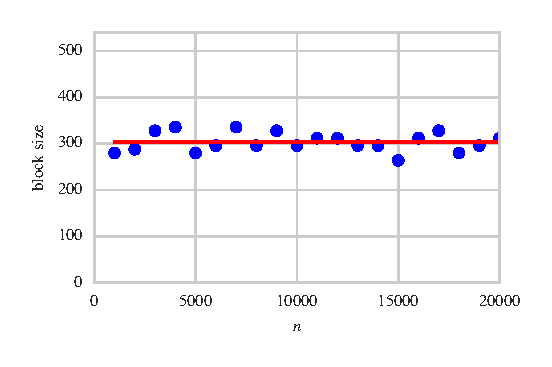
\includegraphics[scale=1]{fig/curvefit_const.eps}
  \caption{The optimal block size for DGEMM is independent of the
    matrix size so a constant model is most appropriate.
    On this architecture the constant is $304$.}
  \label{fig.fit_const}
\end{figure}
%%%%%%%%%%%%%%%%%%%%%%%%%%%%%%
First we investigate the performance of DGEMM
for matrix multiplication.
As we can see from Figure~\ref{fig.fit_const},
the optimal block size is largely independent of the matrix size.
Therefore, we use the mean of all the values to return a constant
block size:
in this case the constant is $304$.
The reason for the lack of dependence on the matrix size is
fairly straightforwards,
since DGEMM is very arithmetic intensive,
involving only fused multiply-adds,
the block size is affected only by the memory hierarchy
and cache size.

%%%%%%%%%%%%%%%%%%%%%%%%%%%%%%
\begin{figure}[ht]
  \centering
  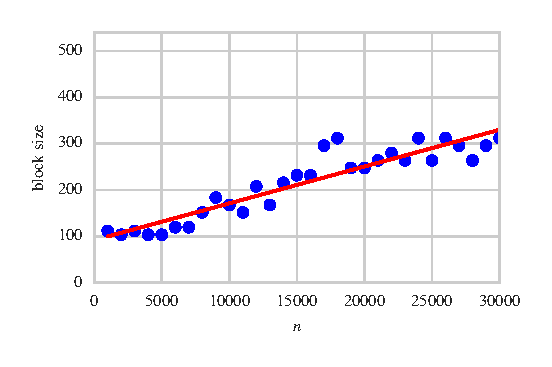
\includegraphics[scale=1]{fig/curvefit_linear.eps}
  \caption{The optimal block size for DGETRF appears to depend
    linearly on the matrix size. In this model the intercept is
    $92.25$ with a gradient of $0.008$.}
  \label{fig.fit_linear}
\end{figure}
%%%%%%%%%%%%%%%%%%%%%%%%%%%%%%
Next we investigate DGETRF for $LU$ factorization
in Figure~\ref{fig.fit_linear}.
In this experiment it is clear that a linear model
provides a much better fit for the data.
Doing a least-squares fit gives an intercept of $92.25$
and a gradient of $0.008$.

%%%%%%%%%%%%%%%%%%%%%%%%%%%%%%
\begin{figure}[ht]
  \centering
  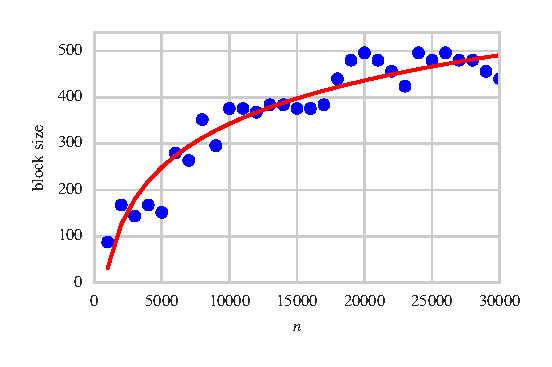
\includegraphics[scale=1]{fig/curvefit_log.eps}
  \caption{The optimal block size for SPOTRF appears to depend
    logarithmically on the matrix size.
    The least-squares fit provides the block size function
    $y = -898 + 135\log(x)$.}
  \label{fig.fit_log}
\end{figure}
%%%%%%%%%%%%%%%%%%%%%%%%%%%%%%
In Figure~\ref{fig.fit_log} we observe that the block size for
SPOTRF (Cholesky factorization in single precision)
increases logarithmically with the matrix size.
The least-squares fit of a model $y = a + b\log(x)$ on
a set of $k$ data points $(x_i, y_i)$ gives the parameters
\begin{align*}
  b &= \frac{k \sum y_i \log(x_i) - \sum y_i \sum \log(x_i)}
            {k \sum\log(x_i)^2 - (\sum \log(x_i))^2},\\
  a &= \frac{\sum y_i - b \sum\log(x_i)}{k}.
\end{align*}
Fitting this model to our data gives the model
$y = -898 + 135 \log(x)$.

%%%%%%%%%%%%%%%%%%%%%%%%%%%%%%
\begin{figure}[ht]
  \centering
  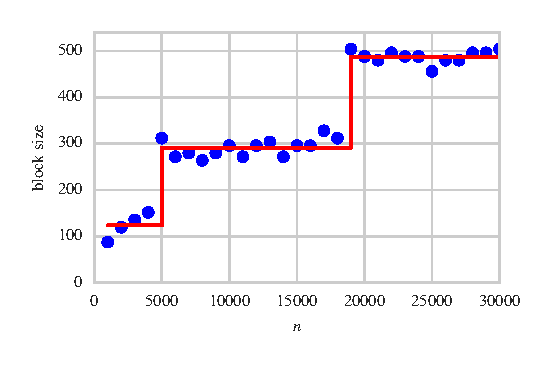
\includegraphics[scale=1]{fig/curvefit_step.eps}
  \caption{The optimal block size for DPOTRF appears to
    be a step function. The three constants in this step function
    are $124$, $291$, and $487$.}
  \label{fig.fit_step}
\end{figure}
%%%%%%%%%%%%%%%%%%%%%%%%%%%%%%
Finally,
by looking at the performance of DPOTRF
(Cholesky factorization in double precision)
in Figure~\ref{fig.fit_step},
we see an example of a routine
where a piecewise function is
the best choice to model the data.
In this particular case a step function is
an appropriate model,
though there are other routines where
initially the function is logarithmic before
settling at some constant value.
In this particular step function the value changes
when the matrix sizes are $5000$ and $19000$,
whilst the three constants are $124$, $291$, and $487$.

In summary there are a variety of different behaviours that
the block size can exhibit depending upon the
routine in question.
Note that even performing the same routine in different
precisions can lead to drastically differing behaviours
(compare Figures~\ref{fig.fit_log}~and~\ref{fig.fit_step}).

As such,
we can only recommend that each routine is treated
independently and no initial assumptions are
made about their behaviour.
Furthermore,
these results are only measured on a Haswell NUMA node.
Moving to more recent architectures,
or the Intel Xeon Phi (codenamed Knights Landing)
may lead to drastically different behaviours.
Clearly,
once these trends have been found,
they need to be coded within Lua functions so that the
software can find the appropriate block sizes at runtime.

%%%%%%%%%%%%%%%%%%%%%%%%%%%%%%
\section{Performance results}
\label{sec.performance}
%%%%%%%%%%%%%%%%%%%%%%%%%%%%%%
\begin{itemize}
\item Try pre/post tuning results vs MKL.
\end{itemize}

%%%%%%%%%%%%%%%%%%%%%%%%%%%%%%
\section{Conclusions}
\label{sec.conclusions}
%%%%%%%%%%%%%%%%%%%%%%%%%%%%%%

\bibliographystyle{plain}
\bibliography{/home/srelton/MATFUN/Total_Bibliography.bib}

%%%%%%%%%%%%%%%%%%%%%%%%%%%%%%%%%%%%%%%%%%%%%%%%%%%%%%%%%%%%
% END OF THE ACTUAL DELIVERABLE
%%%%%%%%%%%%%%%%%%%%%%%%%%%%%%%%%%%%%%%%%%%%%%%%%%%%%%%%%%%%

\end{document}
